\section{Methods}
SciKit-SurgeryFRED implements a simple user interface, Figure \ref{fig:surgery_fred}, to demonstrate registration of a pre-operative image to intra-operative space. At startup a target is placed at a random location within the pre-operative image, shown as a red circle. The standard deviation of the \gls{FLE} is randomly sampled from a uniform distribution 
between 0.5 and 5.0 pixels \footnote{All units are in pixels, as the concepts being explored do not depend on the units used. Figure \ref{fig:surgery_fred} shows a brain MRI 458x512 pixels, by design SciKit-SurgeryFRED should work with other images of arbitrary dimensions.}. By default the \gls{FLE} is modelled as an isotropic (in 3 dimensions), normally distributed, and independent random variable, though this can be easily changed. The variance of the \gls{FLE} is shown at the top left (as expected value), along with number of number of fiducial markers. 

\begin{figure}
	\begin{center}
	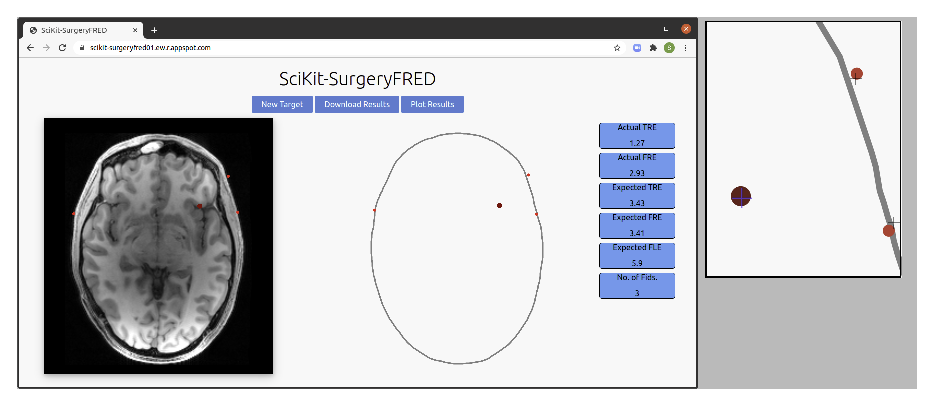
\includegraphics[width=0.9\linewidth]{scikit-surgeryfred_gui.eps}
		\caption{\label{fig:surgery_fred}SciKit-SurgeryFRED graphical user interface after 3 fiducial markers placed. The red sphere in the pre-operative image (left) represents a clinical target, which is located in the
		intra-operative space (middle) by fiducial based registration, using the fiducial markers (green). FLE is added to each marker in the intra-operative image, this is more clearly visible on the zoomed in images at the right. The resulting registration results in a TRE, shown by the misalignment of the red circle and crosshair 
		on the enlarged image at right. TRE and other statistics are shown across the top
		of the window.}
	\end{center}
\end{figure}

Clicking either image adds a fiducial marker to both images. The marker is added to the pre-operative image with no \gls{FLE}. \gls{FLE} is added to the marker location in the intra-operative image, visualised as the misalignment between the green circle centre and the cross-hair. Once sufficient markers are placed ($>2$) the two sets of markers are registered as per \cite{Arun1987}. The expected values (variance) of the \gls{FRE} and \gls{TRE} are calculated 
as per \cite{Fitzpatrick1998}. The registration and statistical algorithms are implemented in SciKit-SurgeryCore \cite{matt_clarkson_2020_3965731}. The student can use this interface together with the
online tutorial 
to explore the relationships between the various statistics and error measures. During use the registration results are 
written to a log file, which can then be used to explore correlation between the different data, an example plot is shown in Figure \ref{fig:correlation}. 
The student should be able to see first hand that, as expected, \gls{FRE} is uncorrelated with \gls{TRE}.

\begin{figure}
	\begin{center}
	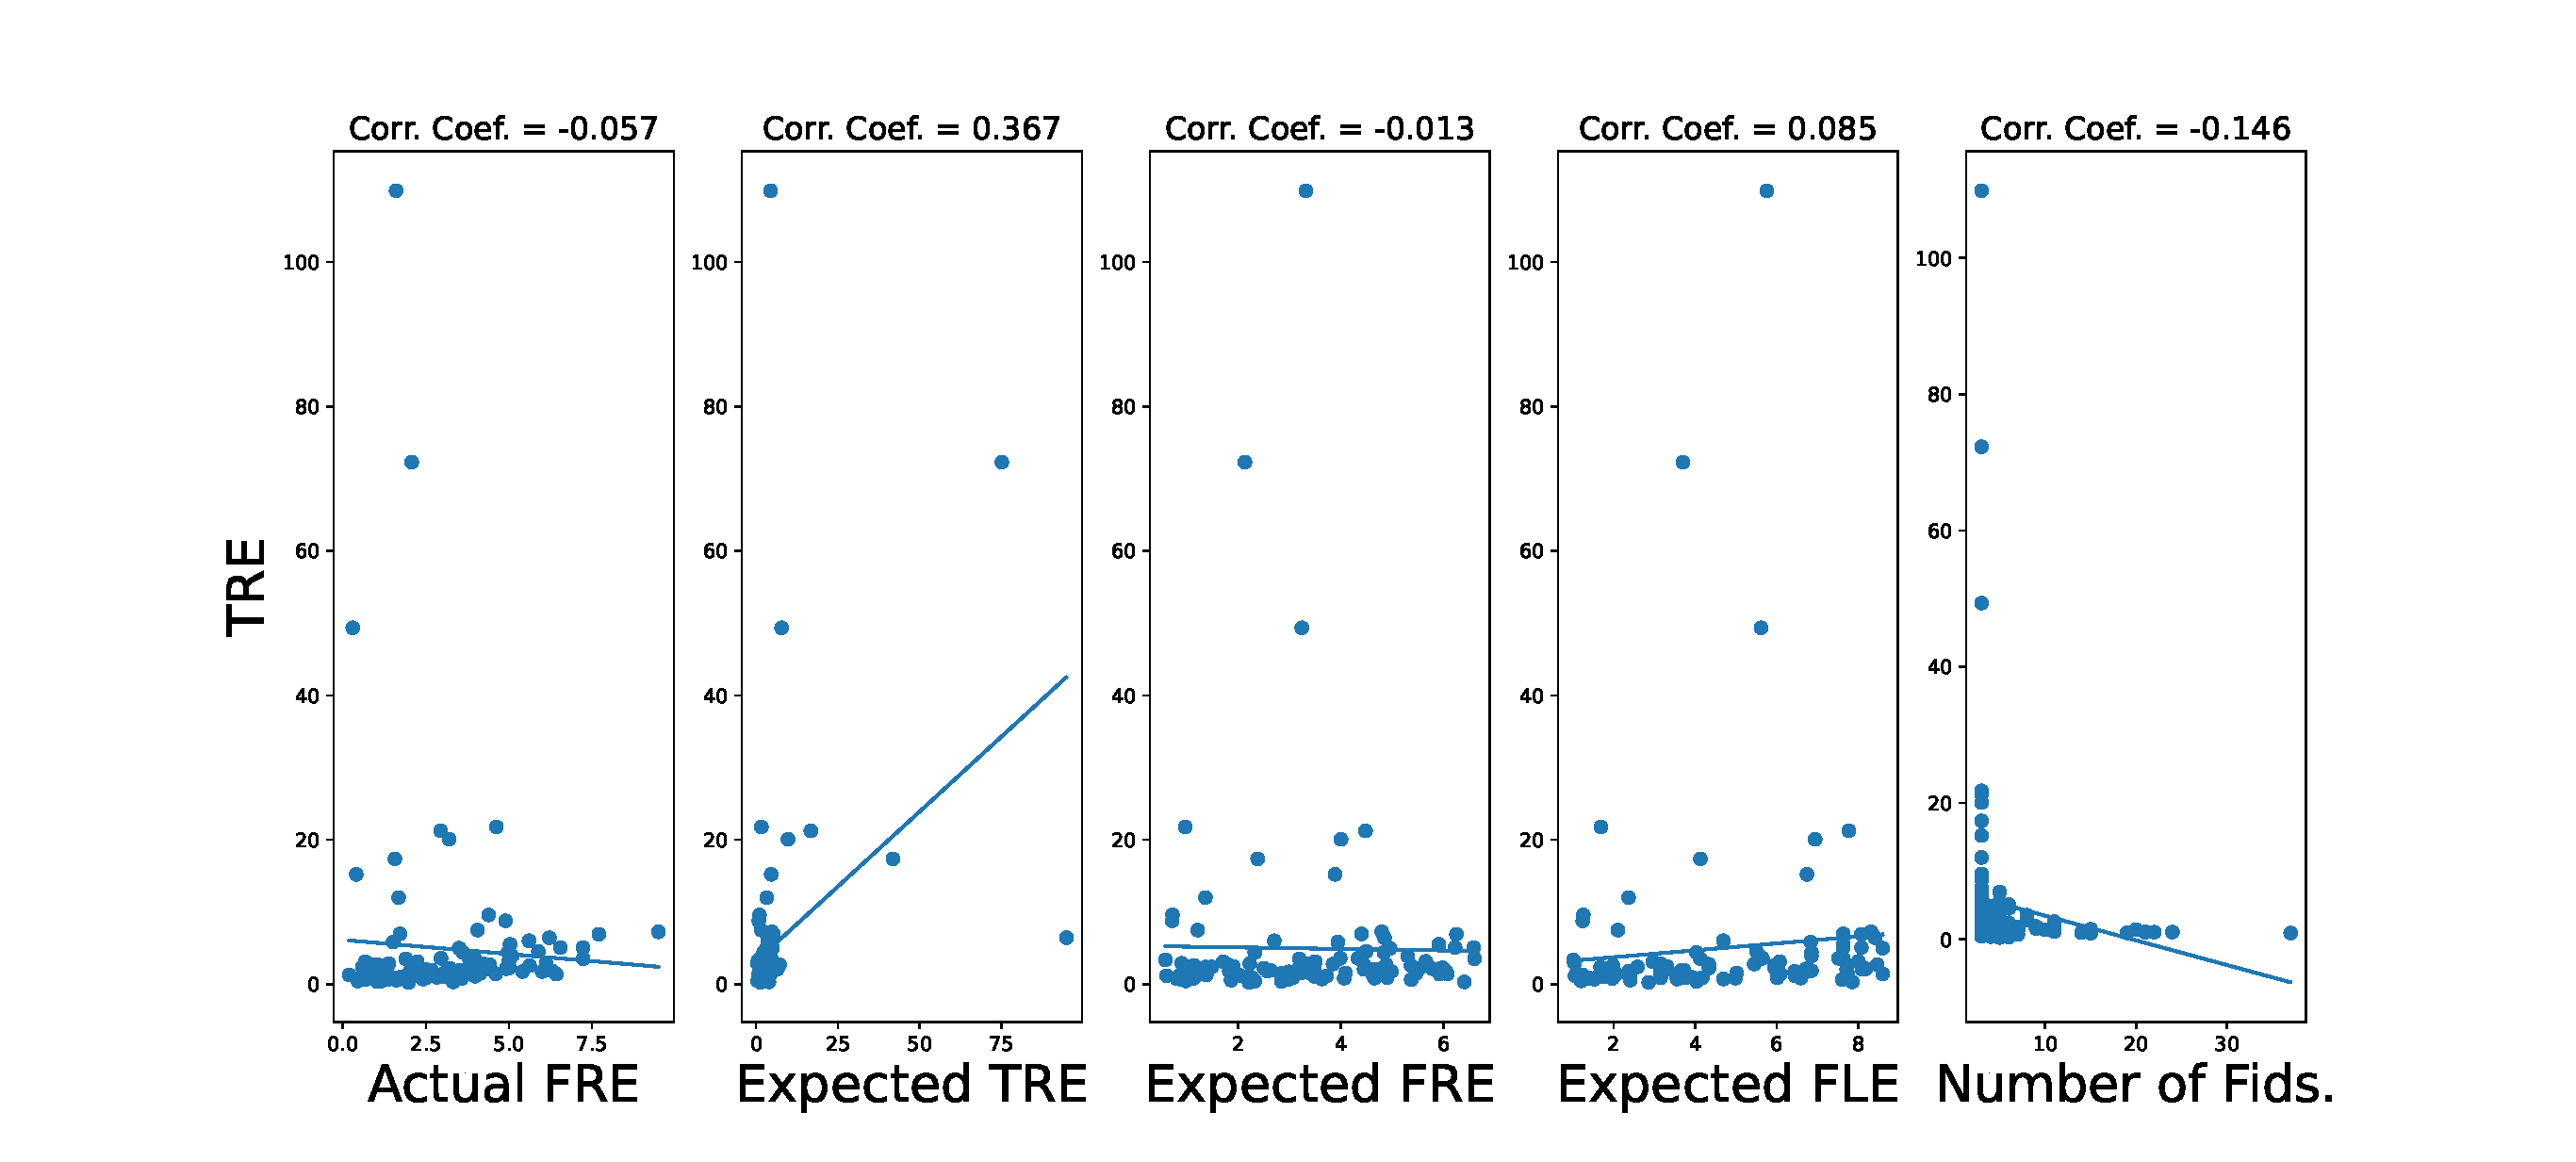
\includegraphics[width=0.9\linewidth]{SciKit-SurgeryF.R.E.D._Correlation_Plots.eps}
		\caption{\label{fig:correlation}Plots of TRE against various error measures, generated by 
		120 user registrations.}
	\end{center}
\end{figure}

\subsection{Game Based Usability Study}
Once the students have an understanding of what statistics can be used to estimate \gls{TRE}, we wanted to test 
how knowledge of a particular statistic affects optimal treatment planning. We designed a serious game to 
do this. After registration the students are able to set a treatment margin and ablate the target. The goal is 
to treat 100\% of the target with minimal ablation of surrounding tissue. A score of 1000 was awarded for 100\% and 0 
for anything less. From this 10 times the percentage volume of any surrounding tissues ablated is subtracted. So 
treatments failing to treat 100\% of the target will receive a negative score. The optimum treatment 
margin is the actual \gls{TRE} for a given registration. 

Each student participated in the game, performing 20 simulated ablations. For the first four ablations they were told the 
actual \gls{TRE}. After that they performed 16 more ablations and were shown one of four randomly selected statistics on which to base their decision,
the expected values of the TRE/FRE, the actual FRE, the expected value of the FLE. Scores were recorded.

